
\section{Striding}
% Authors: Doruk Kilitcioglu, Pedro Manuel Herrero Vidal, Yves Greatti
% Lecture date: 2/25/2019

Striding is a way of subsampling the input to a convolution or a pooling layer such that consecutive operations skip $S-1$ elements between their calculation (Fig. ~\ref{fig:ConvolutionATrou}).
With $S=1$ as default, there will be an output for all inputs, except for the edges.
With $S=2$, there will only be an output for every other input node.
The generalized equation for the resulting number of nodes is
\begin{equation}
    M = \frac{N - K + 1}{2}
\end{equation}

\section{A trou (with holes)}
% Authors: Doruk Kilitcioglu, Pedro Manuel Herrero Vidal, Yves Greatti
% Lecture date: 2/25/2019

A trou is a similar idea to striding, but without the same cost of the resolution decrease.
Instead of skipping between the kernels, a trou skips inside the kernels (Fig. ~\ref{fig:ConvolutionATrou}).
For example, with a trou of 2, one kernel would get input from every other node.
This widens the receptive field of a kernel without subsampling.
The generalized equation for the resulting number of nodes is
\begin{equation}
    M = N - (K-1)S \text{ (ref. \href{https://arxiv.org/pdf/1603.07285.pdf}{A guide to convolution arithmetic for deeplearning})}
\end{equation}
where $S-1$ is the number of holes each kernel leaves while calculating the convolution.
Since the resolution depends on the ratio of output nodes to the input nodes, a trou loses less resolution when compared to striding.

\begin{figure}[!ht]
\centering
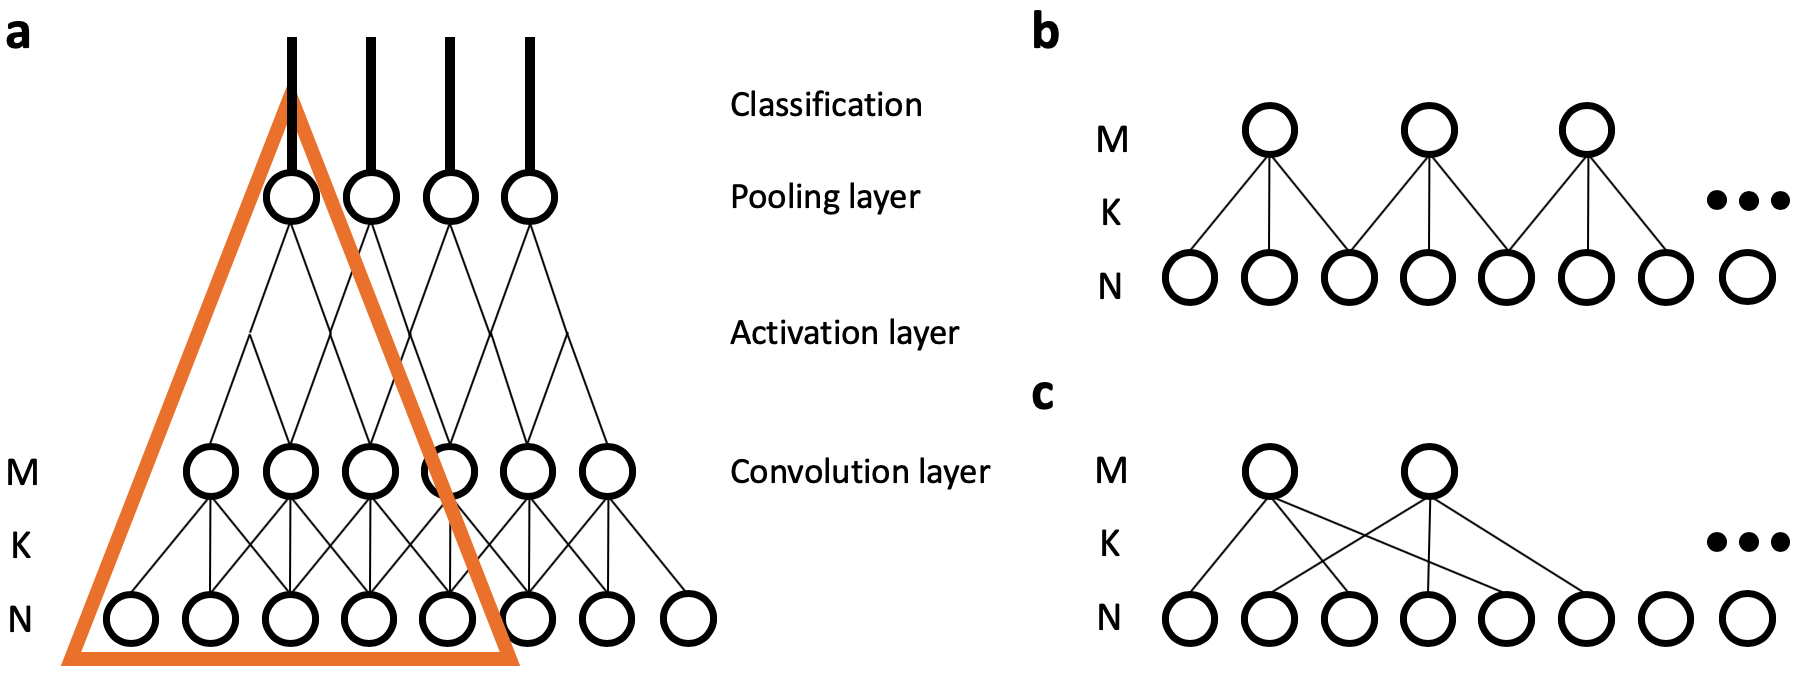
\includegraphics[width=170mm]{figs/ConvolutionATrou.png}
\caption{Types of convolutions in a CNN module. (a) CNN module with input layer of size $N$ a kernel of size $K$ and output $M$, followed by and activation and pooling layers. Convolution with stride $2$ (b) and 'a trou' (c) diagrams.}
\label{fig:ConvolutionATrou}
\end{figure}

\vspace{2mm}
\noindent
In the context of images we want to be able to identify the desired categories independent of location and size. CNN exploit the locality, stationarity and compositionality of the input data using sparsness, parameter sharing and hierarchical structures, respectively. 
Therefore, we can use these networks to not only classify but also locate and segregate data. 
It is doubly beneficial because convolutions are computationally cheap given that we can share parameters for a given convolution kernel (Fig. ~\ref{fig:ConvolutionATrou}, orange selection). Since it is common there is no need to recompute it. It also means that we can only get one output for a particular kernel. So we can apply different kernels to the same input (increasing the depth of the representation) to extract different features. 

\section{Object detection}
% Authors: Doruk Kilitcioglu, Pedro Manuel Herrero Vidal, Yves Greatti
% Lecture date: 2/25/2019

Let's say that we have an object detector that detects objects in an image of 6 pixels.
These 6 pixels are operated on by 4 3x3 kernels to give 4 features.
These four features are operated on by 2 3x3 kernels to give 2 higher level features.
The final layer uses these two features to perform binary classification.

In a larger image, we can slide this object detector over the image to get a probability value of there being our desired object over those pixels. However, if we use a sliding window approach, we do a lot of extra computations because our object detector will re-compute some parts (a whole child branch leading to the output) that were already handled.

Instead we can first apply the first layer of convolutions over the entire image.
From there, we can apply the second batch of convolutions and finally top it off by doing the binary classification.

If we want to emulate a fully connected layer in our object detector, we can use $1\times1$ convolutions.

\section{Uses of object detection}
% Authors: Doruk Kilitcioglu, Pedro Manuel Herrero Vidal, Yves Greatti
% Lecture date: 2/25/2019

\subsection{Word-level training with weak supervision}
% Authors: Doruk Kilitcioglu, Pedro Manuel Herrero Vidal, Yves Greatti
% Lecture date: 2/25/2019

This model introduced the idea of using different window widths to recognize objects (numbers) of different sizes.
Using a sliding window this model can get the probability of a digit occurring over every slice of pixels.

\begin{figure}[!ht]
\centering
	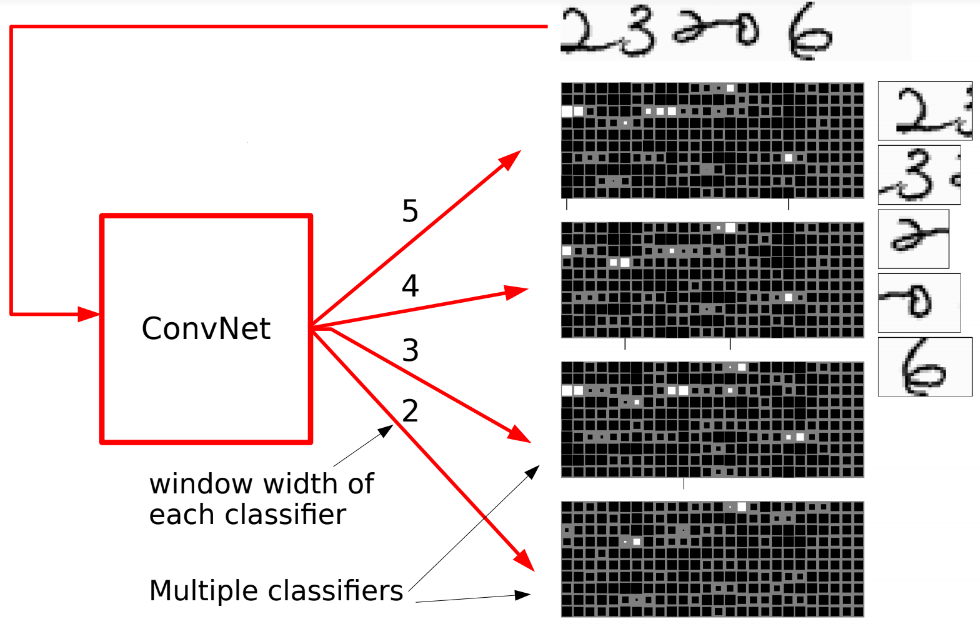
\includegraphics[width=0.5\linewidth]{figs/word-level.png}
	\caption{Digit recognition}
\label{fig:WordLevel}
\end{figure}

When going over a digit, there may be multiple slices of the image where the model gives a high probability of that digit.
In order not to repeat the same digit twice, this model uses a Probabilistic Finite State Machine that combines these probabilities, 
combining regions with high probabilities into one.
This FSM can be solved using the Viterbi algorithm.

\subsection{Face Detection}
% Authors: Doruk Kilitcioglu, Pedro Manuel Herrero Vidal, Yves Greatti
% Lecture date: 2/25/2019

At the time, the largest dataset used for face detection was in around 1000s of examples, instead of the many millions neural networks usually require.
These images were of size $20\times20$, and the neural net used to detect faces was also quite small: there were only two convolutional layers, and a binary output.

The accuracy of this model was also not good, because there were a lot of false positives with images that looked like faces.
In order to increase the accuracy, researchers needed a way of finding negative samples.
The solution was to take a set of images that you knew didn't contain faces and create tons of $20\times20$ batches from those images.
If any of those images gave a false positive, you would add that batch into the set of negative samples.

It should be noted that using white noise as negative sample is not an effective way of training, as the set of all real-life images is only a very small portion of the set of all possible pixel combinations.

This research was unfortunately largely ignored by the computer vision community.

During mid 2000s, research groups realized that detecting if there is a face and the orientation of the face at the same time led to better results compared to doing both tasks separately.
This is called multi-task learning, and it forces the neural net to learn the commonality in between the two tasks.
This acts as a form of regularization, leading to more generalized features for an image.

One other important outcome of this research was the use of non-maximal suppression.
In non-maximal suppression (Fig. ~\ref{fig:NonMaxSupp}), the same image is first subsampled multiple times, creating multiple sizes of the same image.

\begin{figure}[ht]
\centering
	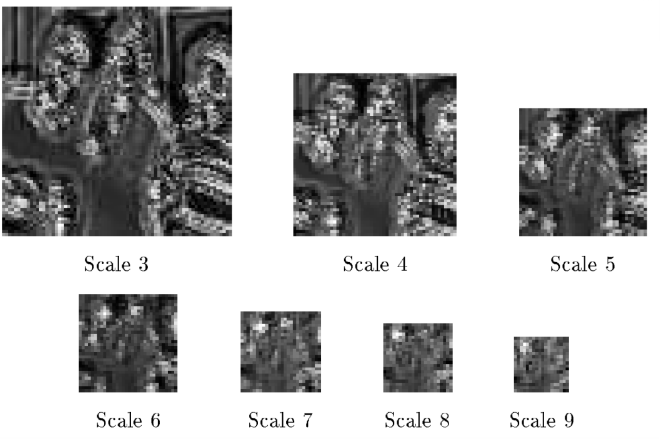
\includegraphics[width=0.5\linewidth]{figs/non-max-supp.png}
	 \caption{Non-maximal suppression}
	\label{fig:NonMaxSupp}
\end{figure}

After this sub-sampling, each kernel goes over each image, generating multiple feature maps.
If there is a partial match in one of the higher resolution images, there is a good chance that there is a perfect match in one of the lower resolution images.
By suppressing all of the non-maximal matches, you can find the right bounding box for an object.
It also allows one kernel to detect the same feature while being size-invariant.



\section{Semantic Segmentation}
% Authors: Doruk Kilitcioglu, Pedro Manuel Herrero Vidal, Yves Greatti
% Lecture date: 2/25/2019

Semantic segmentation looks at the problem of identifying where exactly each object begins and end.
This gives higher fidelity information when compared to using bounding boxes.
Examples include medical imaging for detecting tumors (where you would want to isolate different tumors), and DARPA's LAGR program.

\begin{figure}[ht]
\centering
	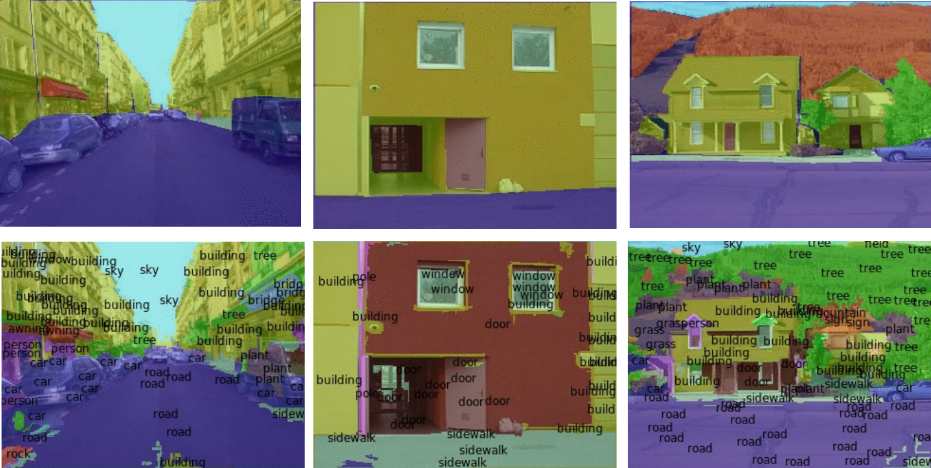
\includegraphics[width=0.8\linewidth]{figs/semantic-segmentation.png}
	\caption{Sematic segmentation}
\label{fig:SemanticSegmentation}
\end{figure}

One way of training these networks is to hand-label each and every pixel with the desired output.

For self-driving vehicles, DARPA's LAGR program used stereo vision, or stereo depth estimation, in order to estimate the relative depth of objects.
Since there is a maximum range you can estimate using stereo vision, LAGR used convolutional nets to estimate longer range depth.
It again used the idea of subsampling to bring down the image to multiple different resolutions before doing the convolution.
This made the convolutional nets more robust (compared to stereo vision) for objects that were near or very far.


Another strategy to produce segmented images is to generate an image of patches using super-pixel to define the boundaries, and then fill each of the patches with the label that is most 'voted' by the network in that section. 

\noindent
To identify categories regardless of location and size, a general recipe would be:
\begin{itemize}
\item[(1)] Use a CNN that takes as input the same imaged but scaled at different resolutions. 
\item[(2)] To prevent false alarms, we retrain the network using a set where the category of interest is not present. We can also incorporate sets with offset focus or non-centered representations of the object. 
\item[(3)] Apply non-maximum suppression. Decide the actual size of the object based on which scale of the image had the best score (or any other metric). 
\end{itemize}
